\documentclass[11pt]{article}
\pdfpxdimen=1in
\divide\pdfpxdimen by 300
 
\usepackage[latin1]{inputenc}
\usepackage[T1]{fontenc}
\usepackage[english]{babel}
\usepackage{mathtools, bm}
\usepackage{amsmath,amssymb,amsthm}
\usepackage{mathrsfs}
\usepackage{cancel}
\usepackage{float}

\usepackage{caption} % to center captions
\usepackage{subcaption} % subcaption for figures side by side

\usepackage{booktabs} % for super cool table
\usepackage[table,xcdraw]{xcolor}  % to put color in tables
\usepackage{tcolorbox} % add box
\usepackage{commath} % for absolute values
\usepackage{stackengine} % to stack things over equal

\usepackage[parfill]{parskip}
\usepackage{graphicx}
\usepackage{hyperref}
\usepackage[top=0.8in, bottom=0.8in, left=1in, right=1in]{geometry}
\usepackage{listings}
\usepackage{framed}

% D( p || q)
\DeclarePairedDelimiterX{\infdivx}[2]{(}{)}{%
  #1\;\delimsize\|\;#2%
}
\newcommand{\infdiv}{D\infdivx}

\renewcommand\thesubsection{\thesection.\arabic{subsection}} % Subsection starting with A, B, ...

\renewcommand\thefigure{\thesubsection.\arabic{figure}}

\newcommand{\horrule}[1]{\rule{\linewidth}{#1}} % Create horizontal rule command with 1 argument of height

\numberwithin{figure}{section} % to have per-section figure numbering

% to use independent and not independent signs %
\makeatletter
\newcommand*{\indep}{%
  \mathbin{%
    \mathpalette{\@indep}{}%
  }%
}
\newcommand*{\nindep}{%
  \mathbin{%                   % The final symbol is a binary math operator
    %\mathpalette{\@indep}{\not}% \mathpalette helps for the adaptation
    \mathpalette{\@indep}{/}%
                               % of the symbol to the different math styles.
  }%
}
\newcommand*{\@indep}[2]{%
  % #1: math style
  % #2: empty or \not
  \sbox0{$#1\perp\m@th$}%        box 0 contains \perp symbol
  \sbox2{$#1=$}%                 box 2 for the height of =
  \sbox4{$#1\vcenter{}$}%        box 4 for the height of the math axis
  \rlap{\copy0}%                 first \perp
  \dimen@=\dimexpr\ht2-\ht4-.2pt\relax
      % The equals symbol is centered around the math axis.
      % The following equations are used to calculate the
      % right shift of the second \perp:
      % [1] ht(equals) - ht(math_axis) = line_width + 0.5 gap
      % [2] right_shift(second_perp) = line_width + gap
      % The line width is approximated by the default line width of 0.4pt
  \kern\dimen@
  \ifx\\#2\\%
  \else
    \hbox to \wd2{\hss$#1#2\m@th$\hss}%
    \kern-\wd2 %
  \fi
  \kern\dimen@
  \copy0 %                       second \perp
}
\makeatother

\title{	
\normalfont \normalsize 
\textsc{Master MVA \\
Probabilistic Graphical Models} \\ [20pt]
\horrule{0.5pt} \\[0.2cm] % Thin top horizontal rule
\textbf{Homework 2}: Classification and Graph Theory \\
\horrule{2pt} \\[0.3cm] % Thick bottom horizontal rule
}

\author{Victor Busa \\
   \texttt{victor.busa@ens-paris-saclay.fr}}

\date{\normalsize\today}

\begin{document}
\def\useanchorwidth{T}

\maketitle

\section{Conditional independence and factorizations}

\paragraph{1.}
We want to prove that: $X \indep Y \,|\; Z$ iff $p(x|y,z) = p(x,z)$ for all pairs $(y,z)$ such that $p(y,z) > 0$, using only:

\begin{align*}
& \textrm{a)} \quad p(x,y|z) = p(x|z)p(y|z) \\
& \textrm{b)} \quad p(x,y) = p(x|y)p(y) \\
& \textrm{c)} \quad \sum\limits_{x} p(x|y) = 1
\end{align*}

\begin{proof}
$  $\newline
$\Rightarrow$ Suppose $p(x,y|z) = p(x|z)p(y|z)$, let's show that $p(x|y,z) = p(x|z)$ for $(y,z)$ s.t $p(y,z) \stackrel{\text{($\Delta$)}}{>} 0$:

\begin{align*}
p(x|y,z) &\stackrel{\text{(b),($\Delta$)}}{=} \frac{p(x,y,z)}{p(y,z)} \stackrel{\text{(b)}}{=} \frac{p(x,y|z)p(z)}{p(y|z)p(z)} = \frac{p(x,y|z)}{p(y|z)} \\
&\stackrel{\text{(a)}}{=} \frac{p(x|z)p(y|z)}{p(y|z)} = p(x|z)
\end{align*}

$\Leftarrow$ Suppose $p(x|y,z) \stackrel{\text{(E)}}{=} p(x|z)$ and $p(y,z) \stackrel{\text{($\Delta$)}}{>} 0$ and let's show that $p(x,y|z) = p(x|z)p(y|z)$:

\begin{align*}
p(x,y|z) &\stackrel{\text{(b)}}{=} \frac{p(x,y,z)}{p(z)} \stackrel{\text{(b)}}{=} \frac{p(x|y,z)p(y,z)}{p(z)} \stackrel{\text{(b)}}{=} \frac{p(x|y,z)p(y|z)p(z)}{p(z)} \\
&= p(y|z)p(x|y,z) \stackrel{\text{(E)}}{=} p(y|z)p(x|z)
\end{align*}

\textbf{Note}: We can divide by $p(z)$, because, by ($\Delta$):

\begin{align*}
p(y,z) > 0 \Rightarrow p(z) \stackrel{\text{(c)}}{=} p(z)\sum\limits_{y} p(y|z) \stackrel{\text{(b)}}{=} \sum\limits_{y} p(y,z) > 0
\end{align*}
\end{proof}

\paragraph{2.}
Let $p \in \mathcal{L}(G)$, then we can write:

$$
p(t,z,x,y) = p(t|z)p(z|x,y)p(x)p(y)
$$

moreover, we have $X \nindep Y \,|\; T$ because we have the d-separation property. Indeed, $T$ is observed and is a child of a V-structure separating $X$ from $Y$.

\paragraph{3.}
\subparagraph{(a)} We want to prove that, assuming $Z$ is a \textbf{binary variable}:

$\left.\begin{tabular}{@{}l@{}}
(1) $p(x,y|z) = p(x|z)$ \\
(2) $p(x,y) = p(x)p(y)$
\end{tabular}\right\}$
$\Rightarrow \Big(p(x,z) = p(x)p(z)\Big)\vee\Big(p(y,z) = p(y)p(z)\Big)$

We notice that we have either $p(x,z) = p(x)p(z)$ or $p(y,z) = p(y)p(z)$, hence we might think, that,
at the end of our demonstration we would have something like: 

$$\left[p(x,z) - p(x)p(z)\right]\left[p(y,z) - p(y)p(z)\right] = 0$$

In order to have something of this form, one good idea is to use 2 different expressions of a certain probability.
Moreover, we will need to use that $Z$ is a \textbf{binary variable}, that is to say: $p(z=1) = 1 - p(z=0)$.
\\
\\
\textbf{Notations}:
\begin{align*}
p(z = 0) &\triangleq p \\
p(z = 0 | X) &\triangleq p_0(X)
\end{align*}

Using our idea, we can write $p(x,y)$ in 2 different ways:

\begin{align}
p(x,y) &= \sum\limits_{z} p(x,y|z)p(z) \stackrel{\text{(1)}}{=} \sum\limits_{z} p(x|z)p(y|z)p(z)\tag{E} \\
p(x,y) &\stackrel{\text{(2)}}{=} p(x)p(y) = \sum\limits_{z}p(x,z)p(z) \sum\limits_{z'} p(y|z')p(z')\tag{E'}
\end{align}

Equating both relations and developing, we have:

\begin{align*}
& (E) = (E') \\
\Leftrightarrow  & \quad p_0(x)p_0(y)p + p_1(x)p_1(y)(1-p) = \Big(p_0(x)p + p_1(x)(1-p)\Big)\Big(p_0(y)p + p_1(y)(1-p)\Big) \\
\Leftrightarrow  & \quad p_0(x)p_0(y)p + \cancel{p_1(x)p_1(y)} - \cancel{p_1(x)p_1(y)p} \\
& = \quad p_0(x)p_0(y)p^2 + p_0(x)p_1(y)p - p_0(x)p_1(y)p^2 + p_1(x)p_0(y)p \\
& - p_1(x)p_0(y)p^2 + \cancel{p_1(x)p_1(y)} - \cancel{2}p_1(x)p_1(y)p + p_1(x)p_1(y)p^2 \\
\Leftrightarrow  & \quad p_0(x)p_0(y)p(p-1) - p_0(x)p_1(y)p(p-1) - p_1(x)p_0(y)p(p - 1) + p_1(x)p_1(y)p(p - 1) = 0 \\
\Leftrightarrow  & \quad p(p - 1)\Big(p_0(x)p_0(y) - p_0(x)p_1(y) - p_1(x)p_0(y) + p_1(x)p_1(y)\Big) = 0 \\
\Leftrightarrow  & \quad p(p - 1)\Big(p_1(y) - p_0(y)\Big)\Big(p_0(x) - p_1(x)\Big) = 0
\end{align*}

Will will consider 3 cases: $p = 0$, $p= 1$ and $0<p<1$:

\begin{tabular}{rl}
\textbf{$p=0$}: & $p(z=0) = 0 \quad\text{and}\quad p(z=1)=1 \quad\text{and}\quad p(z=1) = 1 \Rightarrow p(z=1|x) = 1 = p(z=1)$ \\
\textbf{$p=1$}: & $p(z=0) = 1 \quad\text{and}\quad p(z=1)=0 \quad\text{and}\quad p(z=0) = 1 \Rightarrow p(z=0|x) = 1 = p(z=0)$ \\
if \textbf{$0<p<1$}: & $\Big(p_1(y) - p_0(y)\Big)\Big(p_0(x) - p_1(x)\Big)=0 \quad\text{i.e}\quad p_1(y) = p_0(y) \quad\text{or}\quad p_0(x) = p_1(x)$
\end{tabular}

Hence, if $Z$ is a \textbf{binary variable}, the proposition \\
"If $X \indep Y \,|\; Z$ and $X \indep Y$ then ($X \indep Y$ or $Y \indep Z$)" is \textbf{true}

\subparagraph{(b)} I guess this statement is true in general.

\section{Distributions factorizing in a graph}
\paragraph{1.}
Let's prove that if $G = (V,E)$ is a DAG then we have $\mathcal{L}(G) = \mathcal{L}(G')$  where,
if $i \rightarrow j$ is a covered edge, then we define $E' =  (E\backslash\{i \rightarrow j\})\bigcup\{i \rightarrow j\}$.
To prove this assertion, it suffices to prove that (Figure ~\ref{fig:cover}), if $i \rightarrow j$ is a covered edge, then:

\begin{align*}
p(x_i | x_{\pi_i})p(x_j | x_{\pi_j}) = p(x_i | x_{\pi_i})p(x_j | x_{\pi_i}, x_i) = p(x_j | x_{\pi_i})p(x_i | x_{\pi_i}, x_j)\tag{P}
\end{align*}

\begin{figure}[H]
  \centering
  \begin{minipage}[b]{0.3\textwidth}
    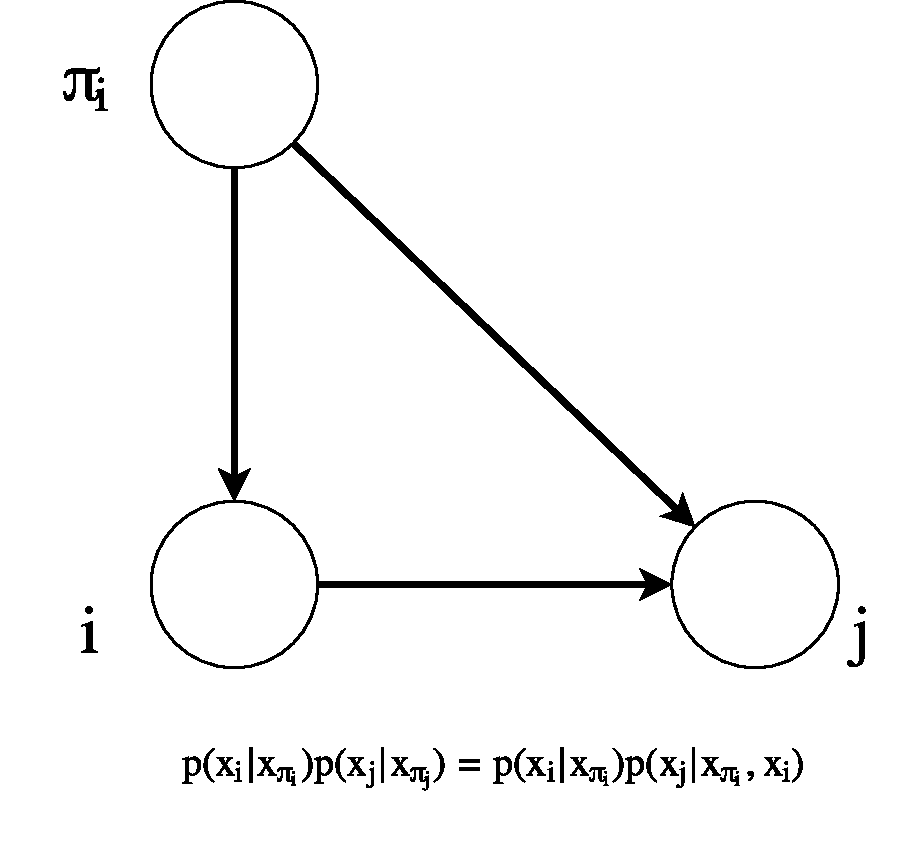
\includegraphics[width=\textwidth]{covered_edge}
    \caption{Edge $(i,j)$ is covered}
  \end{minipage}
  \hfill
  \begin{minipage}[b]{0.3\textwidth}
    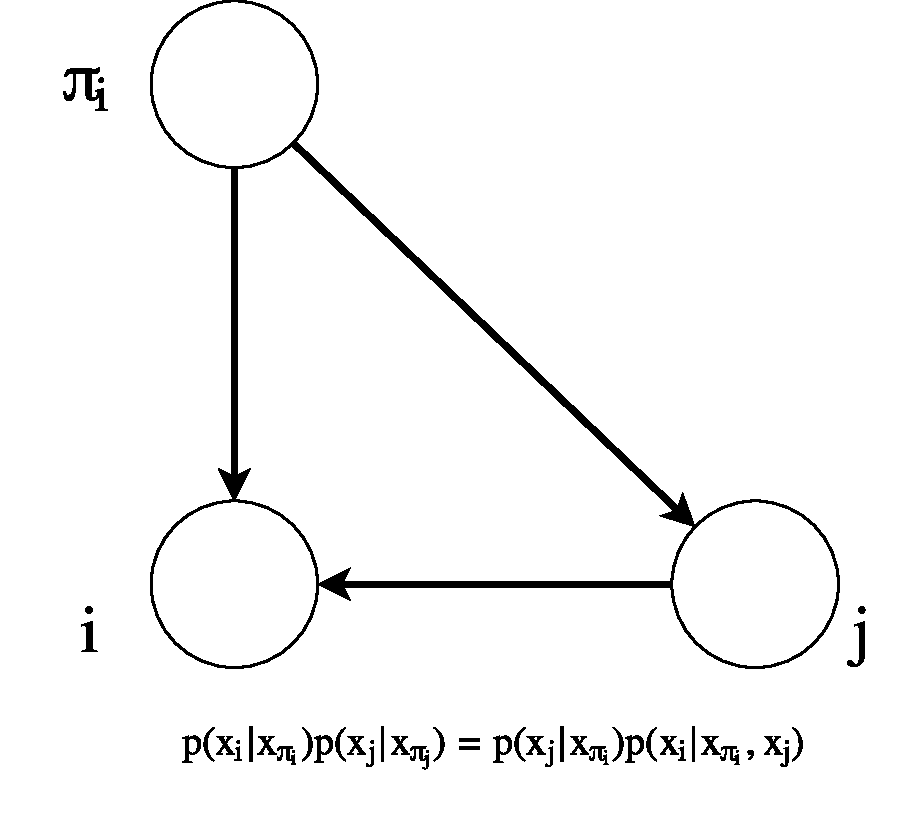
\includegraphics[width=\textwidth]{covered_edge2}
    \caption{Edge $(i,j)$ is reversed}
  \end{minipage}
	\caption{Covered edge and its reverse}
	\label{fig:cover}
\end{figure}

because, in this case $p(x)$ can be written either as (1) or (2).

\begin{align*}
p(x) &= \prod\limits_{k}p(x_k | x_{\pi_k}) \\
&= p(x_i | x_{\pi_i})p(x_j | x_{\pi_j}) \prod\limits_{\substack{k \neq i \\ k\neq j}}p(x_k | x_{\pi_k}) \\
& = p(x_i | x_{\pi_i})p(x_j|x_{\pi_i},x_i)\prod\limits_{\substack{k \neq i \\ k\neq j}}p(x_k | x_{\pi_k})\tag{1} \\
&= p(x_i|x_j, x_{\pi_i})p(x_j|x_{\pi_i}) \prod\limits_{\substack{k \neq i \\ k\neq j}}p(x_k | x_{\pi_k})\tag{2}
\end{align*}

$(1)$ corresponds to $p \in \mathcal{L}(G)$ and $(2)$ corresponds to $p \in \mathcal{L}(G')$. Which proves that $\mathcal{L}(G)=\mathcal{L}(G')$.
So let's prove (P):

\begin{proof}
\begin{align*}
p(x_i | x_{\pi_i})p(x_j | x_{\pi_j}) &= p(x_i | x_{\pi_i})p(x_j|x_{\pi_i},x_i) \\
&= \frac{p(x_i, x_{\pi_i})}{p(x_{\pi_i})} \frac{p(x_j, x_i, x_{\pi_i})}{p(x_i,x_{\pi_i})} \\
&= \frac{p(x_i|x_j, x_{\pi_i})p(x_j|x_{\pi_i})p(x_{\pi_i})}{p(x_{\pi_i})} \\
&= p(x_i|x_j, x_{\pi_i})p(x_j|x_{\pi_i})
\end{align*}
\end{proof}

\paragraph{2.} Let $G$ be a directed tree and $G'$ its corresponding undirected tree, Let's prove that $\mathcal{L}(G) = \mathcal{L}(G')$.\\
\begin{proof}
$ $\newline
To prove that $\mathcal{L}(G) = \mathcal{L}(G')$, we have to express the factorization of p over $\mathcal{L}(G)$ as a factorization of p over $\mathcal{L}(G')$.
A directed tree is a DAG in which all the nodes have exactly \textbf{1 parent} beside the root node that has \textbf{no parent}. If we let $r$ be the root node, $n$
be the number of nodes in the tree and $E = \{(i,j), i \rightarrow j\}$ be the set of all directed edges, we have:

\begin{align*}
p(x) = \prod\limits_{i=1}^n p(x_i | x_{\pi_i}) = p(x_r)\prod\limits_{(i,j) \in E} p(x_j | x_i)
\end{align*}

Indeed, $(i, j)$ being a directed edge, and G being a directed tree, $\{i\} = \pi_j$ is the unique parent of $j$.
If, now, we define:

\begin{align*}
\psi(x_r) &= p(x_r) \\
\psi(x_i) &= 1 \quad \forall i \neq r \\
\psi(x_i, x_j) &=  p(x_j | x_i) \\
Z &= 1
\end{align*}

then we notice that:

\begin{align*}
p(x) &= p(x_r)\prod\limits_{(i,j) \in E} p(x_j | x_i) \\
&= \frac{1}{Z}\left(\prod\limits_{i \in V} \psi(x_i) \prod\limits_{(i,j) \in E} \psi(x_i, x_j) \right)
\end{align*}

which is the factorization of p over G' the undirected tree construct from G, so we have proved that $\mathcal{L}(G) \subset \mathcal{L}(G')$

To  prove that $\mathcal{L}(G') \subset \mathcal{L}(G)$, we can notice that in an undirected tree there is a unique path between every pair of nodes. If we select an arbitrary node to be the root node we can always direct all the edges in the graph to point from the root to the leaf nodes. Moreover every edge in a tree correspond to a two-node potential function that we can replace without loss of generality by a conditional probability distribution provided a certain normalization constant. This conditional probability will only depend on the unique parent of each node as the constructed tree is an directed tree. If the undirected tree doesn't factorize over the directed tree provided our arbitrary choice of the root node, we can, without loss of generality pick another node as the root node. Hence we can replace any undirected tree by N different directed tree where N is the number of nodes of the tree.
\end{proof}

\section{Entropy and Mutual Information}
\paragraph{1.} \subparagraph{(a)} $H(X) \geq 0$ because $\forall x \in \mathcal{X}, \quad 0 \leq p(x) \leq 1$, and hence, $log\, p_X(x) \leq 0$, and so:

\begin{align*}
H(X) = - \sum\limits_{x \in \mathcal{X}} \underbrace{p_X(x)log p_X(x)}_{\leq 0} \geq 0
\end{align*}

Furthermore, $H(X) = 0 \Rightarrow \forall x \in \mathcal{X}, \, p_X(x) log\, p_X(x) = 0$, i.e $\forall x \in \mathcal{X}$,
$p_X(x) = 0$ or $p_X(x) = 1$. Yet, we also have that, $\sum\limits_{x \in \mathcal{X}} p_X(x) = 1$. Hence, $\exists \,x$ s.t $p_X(x) = 1$.
Which proves that $X$ takes one value (hence is constant) with probability 1.

\subparagraph{(b)}
We can compute $\infdiv{p}{q}$ as follow:

\begin{align*}
\infdiv{p}{q} = \sum\limits_{x \in \mathcal{X}} p(x)log\frac{p(x)}{q(x)} = -H(X) - \sum\limits_{x \in \mathcal{X}} p(x) \,log q(x)
\end{align*}
If we let q be the uniform distribution on $\mathcal{X}$, we have: $\sum\limits_{x \in \mathcal{X}} p(x)log \,q(x) = \sum\limits_{x \in \mathcal{X}} p(x)log \frac{1}{\abs{\mathcal{X}}}
= -log \abs{\mathcal{X}}$, because $\sum\limits_{x \in \mathcal{X}} p_X(x) = 1$, so finally we have:

\begin{align*}
\infdiv{p}{q} = -H(X) + log \abs{\mathcal{X}}
\end{align*}

\subparagraph{(c)}
Hence, using question (b) and the fact that $D(p || q) \geq 0$ (seen in class) we have :

\begin{align*}
H(X) \leq log \abs{\mathcal{X}} \triangleq log(k)
\end{align*}

Where we used the notation: $k \triangleq \abs{\mathcal{X}}$

\paragraph{2.}
\subparagraph{(a)}
Let's define $I(X_1, X_2) = \sum\limits_{(x_1,x_2) \in \mathcal{X}_1 \times \mathcal{X}_2} p_{1,2}(x_1,x_2) log \frac{p_{1,2}(x_1,x_2)}{p_1(x_1)p_2(x_2)}$. $I(X_1, X_2) \geq 0$
because we can write: $I(X_1, X_2) = \infdiv{p_{1,2}(X_1, X_2)}{p_1(X_1)p_2(X_2)} \geq 0$ (seen in class).

\subparagraph{(b)}
Let's prove that $I(X_1, X_2)$ can be expressed as a function of $H(X_1)$, $H(X_2)$ and $H(X_1, X_2)$, where $H(X_1, X_2)$ is the entropy of $X = (X_1, X_2)$

\begin{proof}
\begin{align*}
\sum\limits_{(x_1,x_2) \in \mathcal{X}_1 \times \mathcal{X}_2} p_{1,2}(x_1,x_2) log \frac{p_{1,2}(x_1,x_2)}{p_1(x_1)p_2(x_2)} &=
\sum\limits_{(x_1,x_2) \in \mathcal{X}_1 \times \mathcal{X}_2} p_{1,2}(x_1,x_2) log \,p_{1,2}(x_1,x_2) \;- \\ 
&\sum\limits_{(x_1,x_2) \in \mathcal{X}_1 \times \mathcal{X}_2} p_{1,2}(x_1,x_2) log \,p_1(x_1)p_2(x_2) \\
&= \sum\limits_{(x_1,x_2) \in \mathcal{X}_1 \times \mathcal{X}_2} p_{1,2}(x_1,x_2) log \,p_{1,2}(x_1,x_2) \;- \\
&\sum\limits_{(x_1,x_2) \in \mathcal{X}_1 \times \mathcal{X}_2} p_{1,2}(x_1,x_2) log \,p_1(x_1) \;- \\
&\sum\limits_{(x_1,x_2) \in \mathcal{X}_1 \times \mathcal{X}_2} p_{1,2}(x_1,x_2) log \,p_2(x_2)
\end{align*}

furthermore, we have:

\begin{align*}
\sum\limits_{(x_1,x_2) \in \mathcal{X}_1 \times \mathcal{X}_2} p_{1,2}(x_1,x_2) log \,p_2(x_2) &= 
\sum\limits_{x_2 \in \mathcal{X}_2} log \,p_2(x_2) \sum\limits_{x_1 \in \mathcal{X}_1} p_{1,2}(x_1,x_2) \\
&= \sum\limits_{x_2 \in \mathcal{X}_2} log \,p_2(x_2) p_{2}(x_2) = -H(X_2)
\end{align*}

And in the same way,

\begin{align*}
\sum\limits_{(x_1,x_2) \in \mathcal{X}_1 \times \mathcal{X}_2} p_{1,2}(x_1,x_2) log \,p_1(x_1) = -H(X_1)
\end{align*}

so, finally, we can rewrite $I(X_1, X_2)$ as:

\begin{align*}
I(X_1, X_2) = - H(X_1, X_2) + H(X_1) + H(X_2)
\end{align*}
\end{proof}

\subparagraph{(c)}
Using the previous questions we have that: $I(X_1, X_2) = - H(X_1, X_2) + H(X_1) + H(X_2) \geq 0$, i.e

\begin{align*}
H(X_1, X_2) \leq H(X_1) + H(X_2)
\end{align*}

And we have equality when $X_1 \indep X_2$, i.e the maximal entropy is such that: $p_{1,2}(x_1, x_2) = p_1(x_1)p_2(x_2)$

\section{Implementation - Gaussian mixtures}
\paragraph{(a)} See code for the implementation of K-means. The Figure ~\ref{fig:hist} displays the histograms of distortion for $500$ random initializations. The Figure ~\ref{fig:kmeans1} displays the clusters and distortion for a certain random initialization. The
Figure ~\ref{fig:kmeans2} displays two more clusters and distortion curve for 2 more random initialization. 

\begin{figure}[H] 
	\centering
	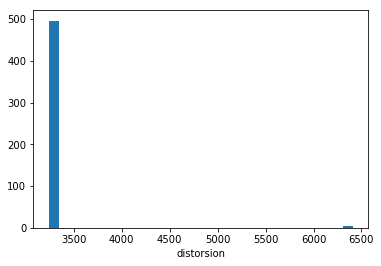
\includegraphics[scale=0.8]{images/histo.png}
	\caption{histograms of the distortion for $500$ random initialization}
	\label{fig:hist}
\end{figure}

\begin{figure}[H] 
	\centering
	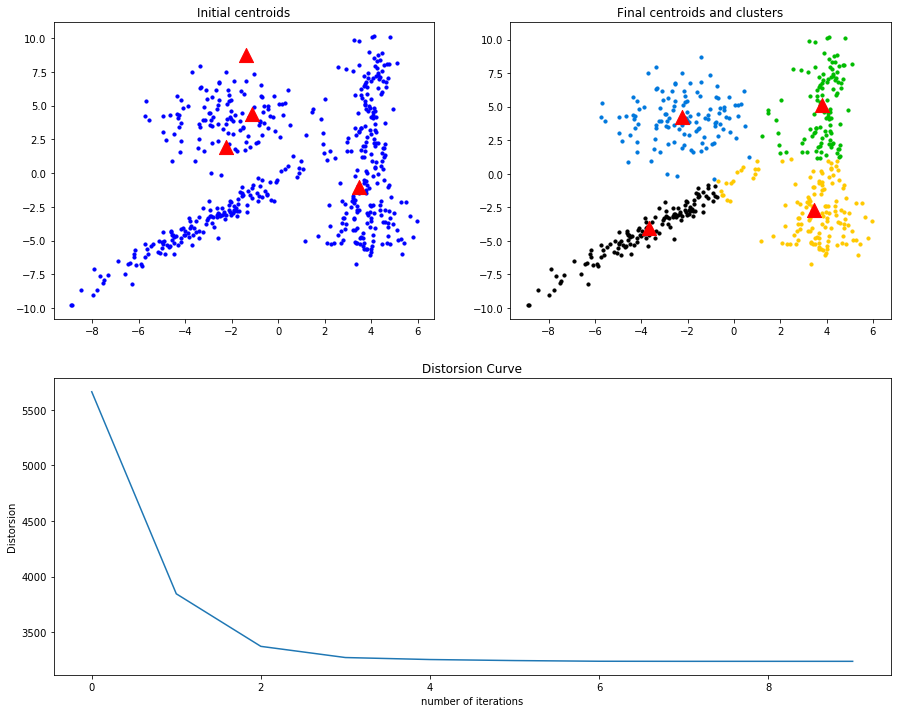
\includegraphics[scale=0.5]{images/kmeans_1.png}
	\caption{clusters and distortion for one random initializations}
	\label{fig:kmeans1}
\end{figure}

We can see that, in our experiment, K-means converges to the same near optimal centroids \textbf{in most of the case}$^{~\ref{fig:hist}}$ $^{~\ref{fig:bad_kmeans}}$. Yet we've also noticed that for some bad random initialization K-means doesn't converge to a good nearly optimal solution. Hence we must carefully check that K-means has converged to a nearly optimal solution.

\paragraph{(b)}
Let $(x_i, z_i)$ be a couple, for $i \in \{1, \hdots, n\}$ with $x_i \in \mathbb{R}^2$, $z_i \sim \mathcal{M}(1, \pi_1,... \pi_K)$ and $(x_i | z_i = k) \sim \mathcal{N}(\mu_k, \Sigma_k)$.
Here, the parameters are: $\theta = (\pi, \mu, \Sigma)$. To derive the \textbf{E}xpectation Step and the \textbf{M}aximization Step, we will write the c\textbf{}omplete log-likelihood at the time step \textbf{t}, and we note $\ell_{c,t}$:

\begin{align*}
\ell_{c,t} = log \; p(x, z; \theta_t) &= \sum\limits_{i=1}^n log \; p(x_i, z_i; \theta_t) \\
&= \sum\limits_{i=1}^n log \; p(z_i; \theta_t)p(x_i | z_i; \theta_t) \\
&= \sum\limits_{i=1}^n log \; p(z_i; \theta_t) + \sum\limits_{i=1}^n log \; p(x_i | z_i; \theta_t) \\
&= \sum\limits_{i=1}^n \sum\limits_{k=1}^K \delta_{i, k} log \; p(\pi_{k,t}) + \sum\limits_{i=1}^n \sum\limits_{k=1}^K \delta_{i, k} log \; \mathcal{N}(x_i, \mu_{k,t}, \Sigma_{k,t})
\end{align*}

\textbf{E-Step}: We need to write the Expectation of $\ell_{c,t}$ w.r.t $(Z|X)$. i.e:

\begin{align*}
\mathbb{E}_{(Z|X)}[\ell_{c,t}] &= \mathbb{E}\left[\sum\limits_{i=1}^n \sum\limits_{k=1}^K \delta_{i, k} log \; p(\pi_{k,t}) + \sum\limits_{i=1}^n \sum\limits_{k=1}^K \delta_{i, k} log \; \mathcal{N}(x_i, \mu_{k,t}, \Sigma_{k,t})\right] \\
&= \sum\limits_{i=1}^n \sum\limits_{k=1}^K \mathbb{E}_{(Z|X)}[\delta_{i, k}] log \; p(\pi_{k,t}) + \sum\limits_{i=1}^n \sum\limits_{k=1}^K \mathbb{E}_{(Z|X)}[\delta_{i, k}] log \; \mathcal{N}(x_i, \mu_{k,t}, \Sigma_{k,t})
\end{align*}

So, we only need to compute $\mathbb{E}_{(Z|X)}[\delta_{i, k}]$. But $\mathbb{E}_{(Z|X)}[\delta_{i, k}] = p(z_i = k | x_i; \theta_t)$. So we need to compute $p(z_i = k | x_i; \theta_t)$.
As seen in class, we have the relation:

\begin{align*}
p(z_i = k | x_i; \theta_t) &= \frac{\pi_k \mathcal{N}(x_i | \mu_k, \Sigma_k)}{\sum\limits_{k^{\prime}} \pi_{k\prime} \mathcal{N}(x_i | \mu_{k^{\prime}}, \Sigma_{k^{\prime}})} \\
\triangleq \tau^{k}_i
\end{align*}

\textbf{M-Step}: We need to maximize the following quantity with respect to $\theta_t = (\pi_t, \mu_t, \Sigma_t)$:

\begin{align}
\sum\limits_{i=1}^n \sum\limits_{k=1}^K \tau^{k}_i log \; p(\pi_{k,t}) + \sum\limits_{i=1}^n \sum\limits_{k=1}^K \tau^{k}_i log \; \mathcal{N}(x_i, \mu_{k,t}, \Sigma_{k,t})
\end{align}

The calculation of the maximization of (1) w.r.t $\theta_t = (\pi_t, \mu_t, \Sigma_t)$ has been seen in class. The only difference in the isotropic case is the calculation of $\Sigma_{k,t}$ ($\Sigma$ w.r.t the $k^{th}$ cluster at time step t). In the Isotropic case we have $\Sigma_{k,t} = \sigma_{k,t} I$, such that:

\begin{align*}
\mathcal{N}(x_i|u_{k,t}, \Sigma_{k,t}) = \frac{1}{(2\pi)^{d/2}\sigma_{k,t}^{d/2}}
exp\left(\frac{-1}{2\sigma_{k,t}}(x_i - \mu_{k,t})^{\intercal}(x_i - \mu_{k,t})\right)
\end{align*}

As we want to maximize $\sigma_{k}$ at time step $t+1$, we need to compute the value
of $\sigma_{k,t+1}$ for which $\nabla_{\sigma_k}\left(\sum\limits_{i=1}^n\sum\limits_{k=1}^K \tau^{k}_i log\; \mathcal{N}(x_i|u_{k,t}, \Sigma_{k,t})\right) = 0$:

\begin{align*}
\nabla_{\sigma_k}\left(\sum\limits_{i=1}^n\sum\limits_{k=1}^K \tau^{k}_i (C - log(\sigma^{d/2}_{k}) - \frac{1}{2 \sigma_k}(x_i - \mu_{k})^{\intercal}(x_i - \mu_{k}))\right) = 0\\
\Leftrightarrow \sum\limits_{i=1}^n -\frac{d}{2 \sigma_k}\tau^{k}_i + \frac{1}{2 \sigma^2_k} \tau^{k}_i (x_i - \mu_{k})^{\intercal}(x_i - \mu_{k}) = 0 \\
\Leftrightarrow \sigma_k = \frac{1}{d}\frac{\sum\limits_{i=1}^n \tau^{k}_i \norm{x_i - \mu_k}^2_2}{\sum\limits_{i=1}^n \tau^{k}_i}
\end{align*}

So finally, in the isotropic case, the update becomes:

\begin{framed}
\begin{align*}
\sigma_{k,t+1} = \frac{1}{d}\frac{\sum\limits_{i=1}^n \tau^{k}_{i,t} \norm{x_i - \mu_{k,t}}^2_2}{\sum\limits_{i=1}^n \tau^{k}_{i,t}}
\end{align*}
\end{framed}


The Figure ~\ref{fig:isotropic_em} displays the clusters, the centroids and the 4 gaussians centered on the centroids. We can see that this model doesn't fit well the data as the clusters are approximated by circles due to the isotropic covariance. Isotropic Gaussian mixture seems to behave like K-means due to the fact that it doesn't take into account the correlation between the variables.

\begin{figure}[H] 
	\centering
	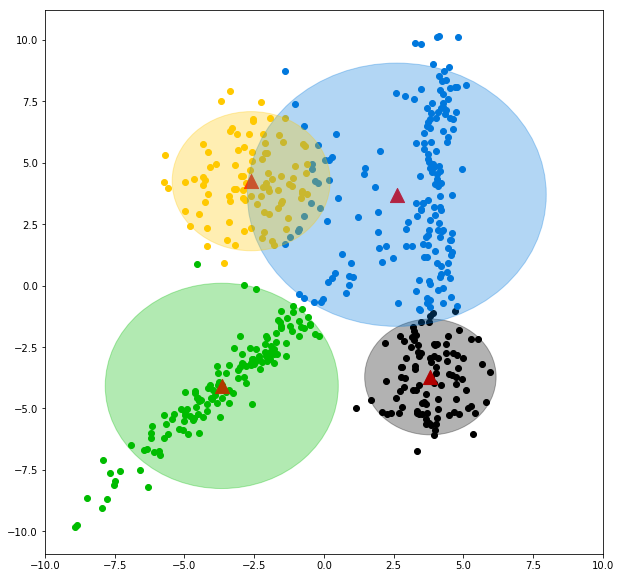
\includegraphics[scale=0.5]{images/isotropic_em.png} % width=1\linewidth
	\caption{EM with isotropic covariance and $K=4$}
	\label{fig:isotropic_em}
\end{figure}


\paragraph{(c)}
The Figure ~\ref{fig:general_em} displays the clusters, the centroids and the 4 gaussians centered on the centroids. We can see that this model fits the data quite well. Indeed the data seems to have been generated by 4 Gaussians with different non isotropic covariance. Hence, as we removed the assumption that the covariance is isotropic, the clusters can be any kind of ellipses and that is why this model performs well.

\begin{figure}[H] 
	\centering
	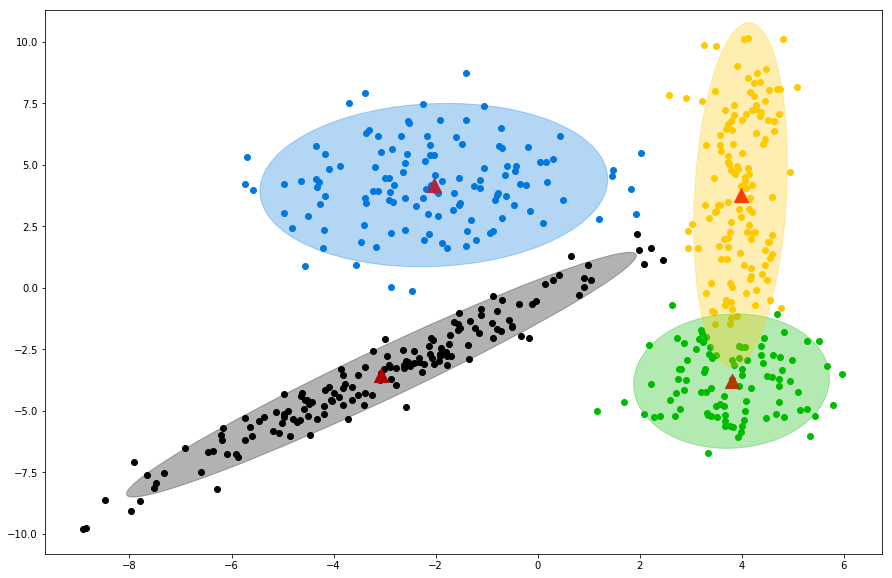
\includegraphics[width=1\linewidth]{images/general_em.png}
	\caption{EM with isotropic covariance and $K=4$}
	\label{fig:general_em}
\end{figure}

\paragraph{(d)}

The results are summarized in Table ~\ref{table:loglike} below

\begin{table}[H]
\centering
\begin{tabular}{|l|l|l|}
\hline
\textbf{} & \multicolumn{2}{c|}{\textbf{log-likelihood}} \\ \hline
\textbf{model} & Training set & Testing set \\ \hline
Isotropic & -2639.56 & -2614.60 \\ \hline
General & -2327.72 & -2408.97 \\ \hline
\end{tabular}
\caption{Log-likelihood of the two mixture models for the Training and Testing set}
\label{table:loglike}
\end{table}

As expected, the log-likelihood of the general mixture model is smaller than the log-likelihood of the isotropic model. Hence, the general model
outperforms the isotropic model. We can also notice that the log-likelihood on the Testing set is slightly lower than on the Training set for the isotropic case, which is
quite unusual. This can be easily explains by the fact that the data have surely been randomly generated using a mixture of Gaussians. \\
Finally it is much more informative to return the normalized log-likelihood (as \texttt{scikit-learn} does) i.e the log-likelihood divided by the number of samples (here 500).

\section{Annexe}

\begin{figure}[H]
\centering
	\begin{subfigure}[b]{.75\textwidth}
		\centering
		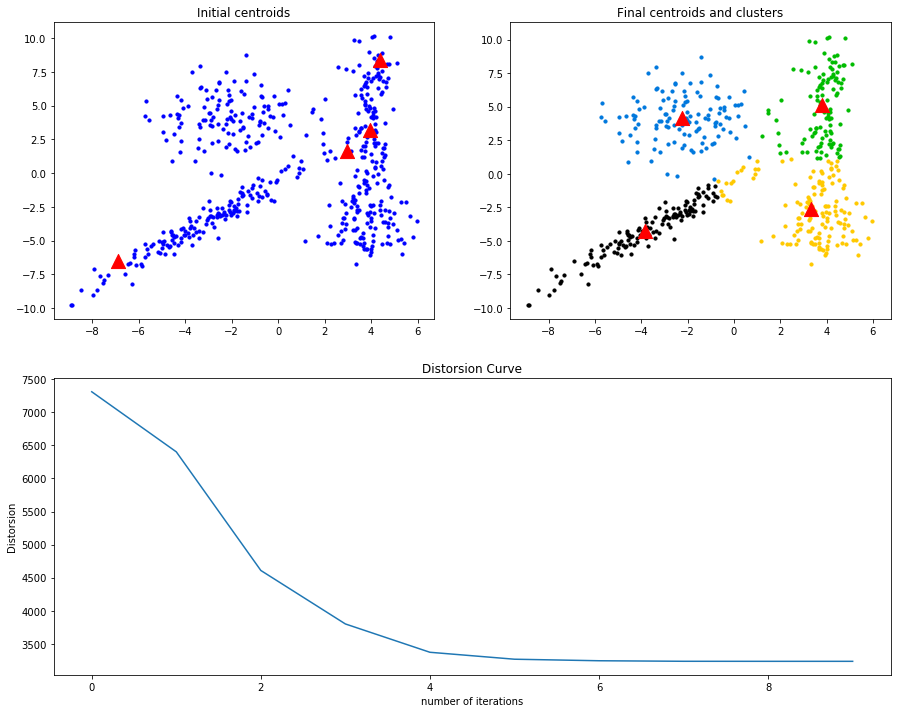
\includegraphics[width=1\linewidth]{images/kmeans_2.png}
		\label{fig:kmeansa}
	\end{subfigure}
	\begin{subfigure}[b]{.75\textwidth}
		\centering
		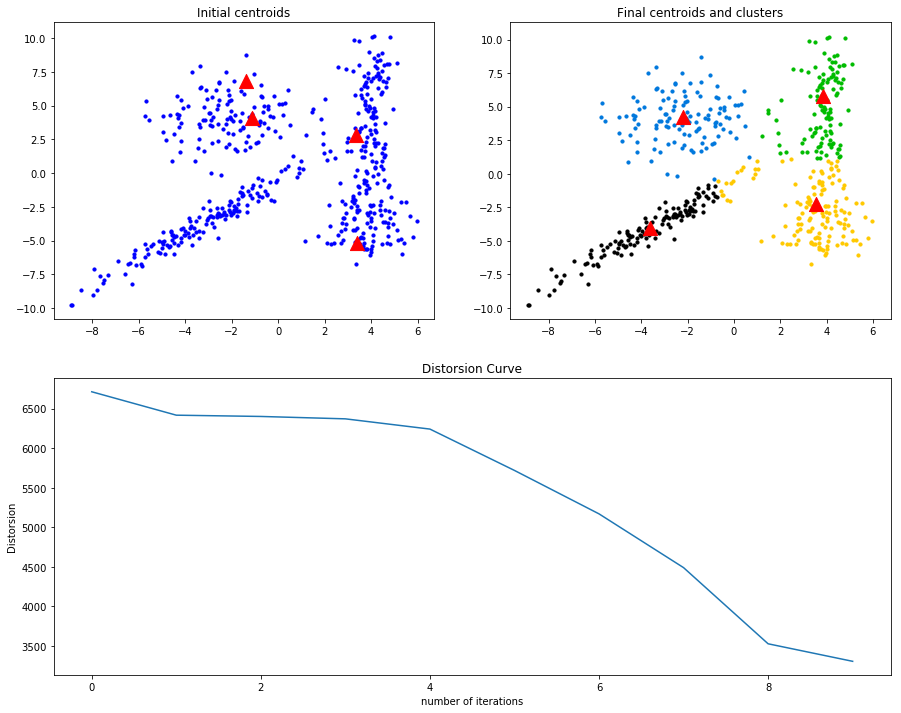
\includegraphics[width=1\linewidth]{images/kmeans_3.png}
		\label{fig:kmeansb}
	\end{subfigure}
\caption{clusters and distortion for 2 more random initialization}
\label{fig:kmeans2}
\end{figure}

\begin{figure}[H] 
	\centering
	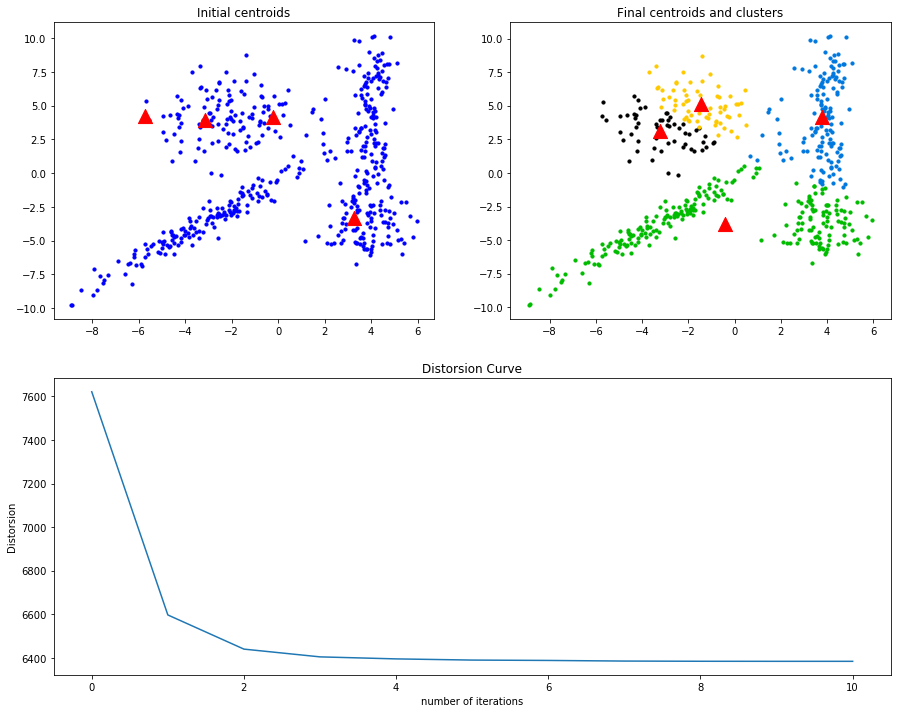
\includegraphics[width=1\linewidth]{images/bad_case.png}
	\caption{clusters and distortion for a bad random initialization}
	\label{fig:bad_kmeans}
\end{figure}

\end{document}
